\documentclass[deutsch]{scrartcl}
\usepackage[ngerman]{babel}
\usepackage[utf8]{inputenc}
\usepackage{algorithmic}
\usepackage{algorithm}
\usepackage{graphicx}
\usepackage{amsmath,amssymb}
\usepackage{subcaption}
\captionsetup{compatibility=false}
\usepackage{multirow}
\usepackage{color}

\begin{document}

\title{Konzept: Schnapskönig} %%Projekttitel hier eintragen

\subtitle{EDBV WS 2017/2018: AG\_A2} %%statt XX Arbeitsgruppenbezeichnung hier eintragen (zB.: A1)


%%Namen und Matrikelnummern der Gruppenmitglieder hier eintragen
\author{Jan Michael Lajarno (01425799)\\
Andreas Brunner (01429369)\\
Miran Jank (01526438)\\
Thorsten Korpitsch (01529243)\\
Aleksandar Marinkovic (01634028)\\
}



%%------------------------------------------------------

\maketitle


%%------------------------------------------------------

\section{Ziel}
\textit{Der Gewinner einer Runde wird erkannt(der Stich) und die Punkte werden dem Gewinner zugerechnet. Am Ende wird der Gewinner gekührt.}
\section{Eingabe}
\textit{Der Benutzer muss nur ein Farbbild, in einem gängigen Format(.PNG/.JPG/.JPEG), der Karten, des aktuellen Spielzugs, bereitstellen.}
\section{Ausgabe}
\textit{In der Konsole wird ein Zwischenstand nach jeder Runde ausgegeben, am Ende wird der Gewinner ausgegeben und der Endstand.}
\section{Voraussetzungen und Bedingungen}
\textit{Ein Farbbild der Karten. Der Hintergrund sollte möglichst Einfarbig sein (nicht weiß, texturarm). Die Kamera soll sich in einem Winkel von 45 bis 135 Grad befinden. Die Karten müssen mit einem dünnen schwarzen Rand preperiert sein.}
\section{Methodik}
\begin{enumerate}
	\item Geometrische Transformation: Um das Eingabebild vorzubereiten wird aus dem, bis zu 45 Grad schrägen Bild, ein Bild aus der Vogelperspektive (90 Grad) transformiert
	\item Kanten-Filter: Um die einzelnen Spielkarten zu trennen wird eine Kantendetektion durchgeführt
	\item Template-Matching: Um die Spielkarte zu identifizieren wird ein Pattern-Matching durchgeführt
\end{enumerate}
\section{Evaluierung}
\begin{itemize}
	\item Wird das Bild richtig transformiert, oder werden Buchstaben/Symbole verzerrt?
	\item Werden beide Karten erkannt?
	\item Wird die Karte richtig identifiziert?
\end{itemize}
\section{Datenbeispiel}
\begin{figure}[h!]
 \centering
 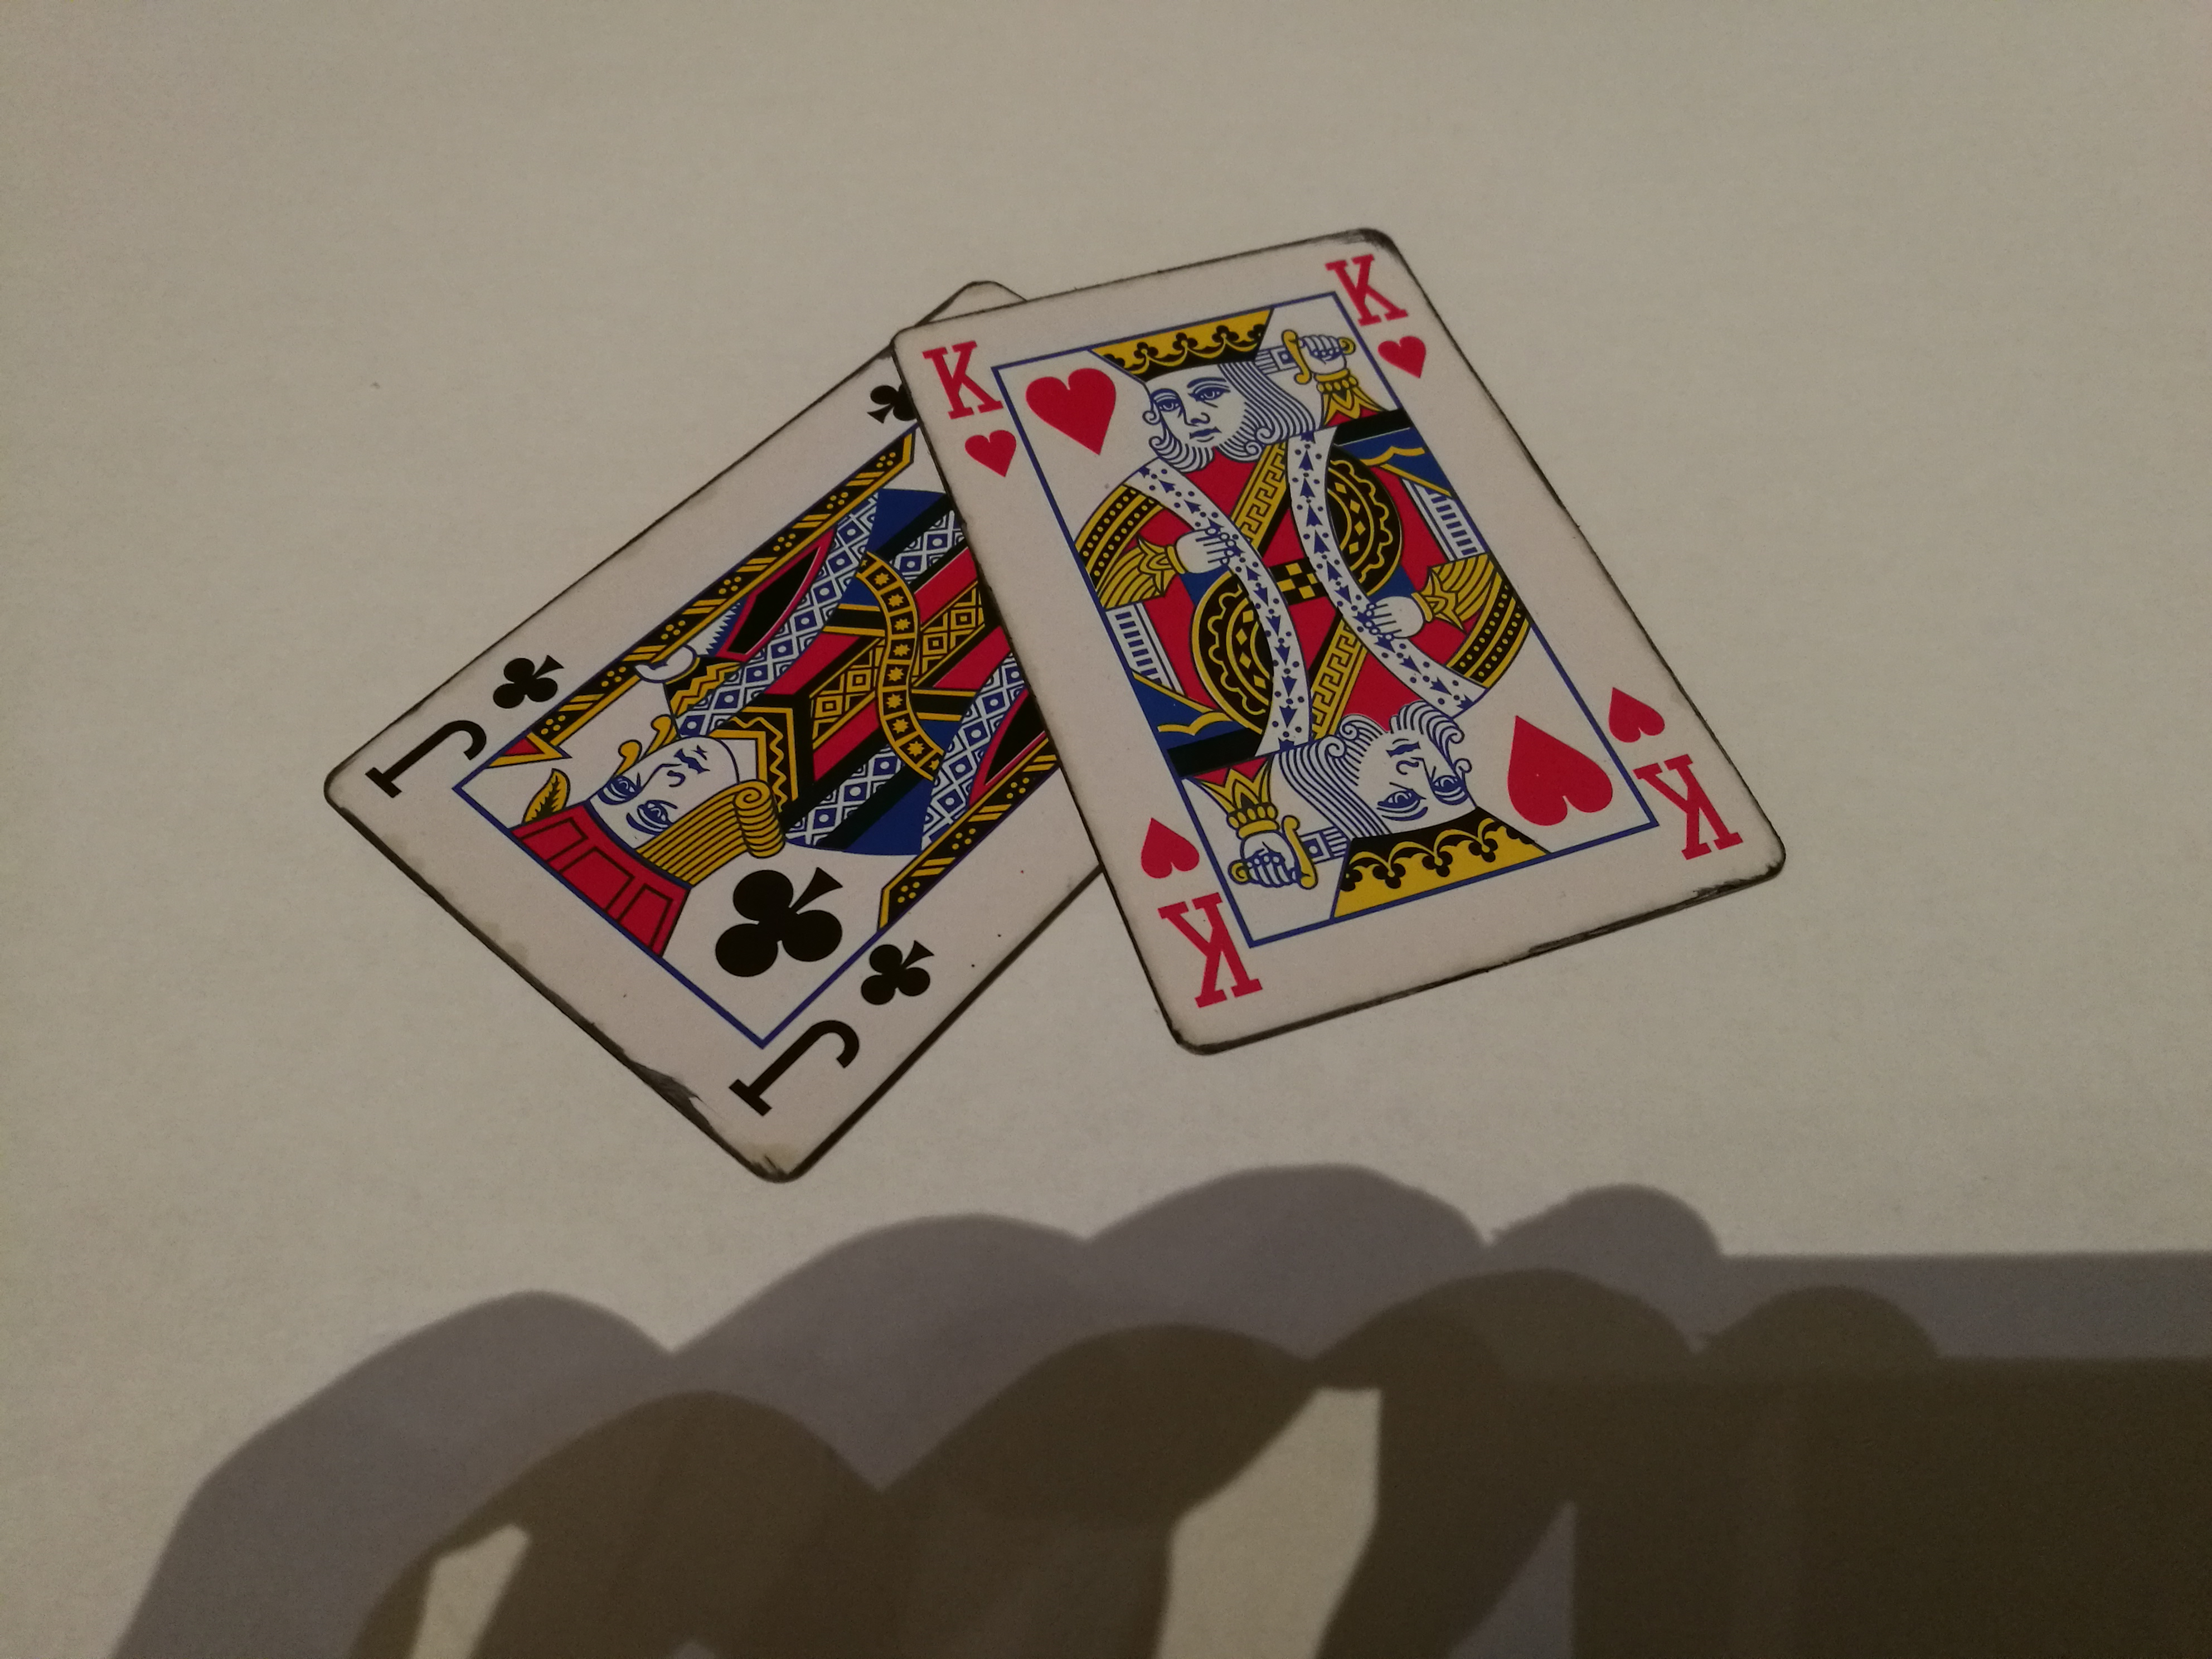
\includegraphics[width=0.4\textwidth]{datenbeispiel.jpg}
 \caption{Kreuz-Bube sticht Herz-König, 6 Punkte gewonnen}
 \label{fig:img}
\end{figure}
\begin{figure}[h!]
 \centering
 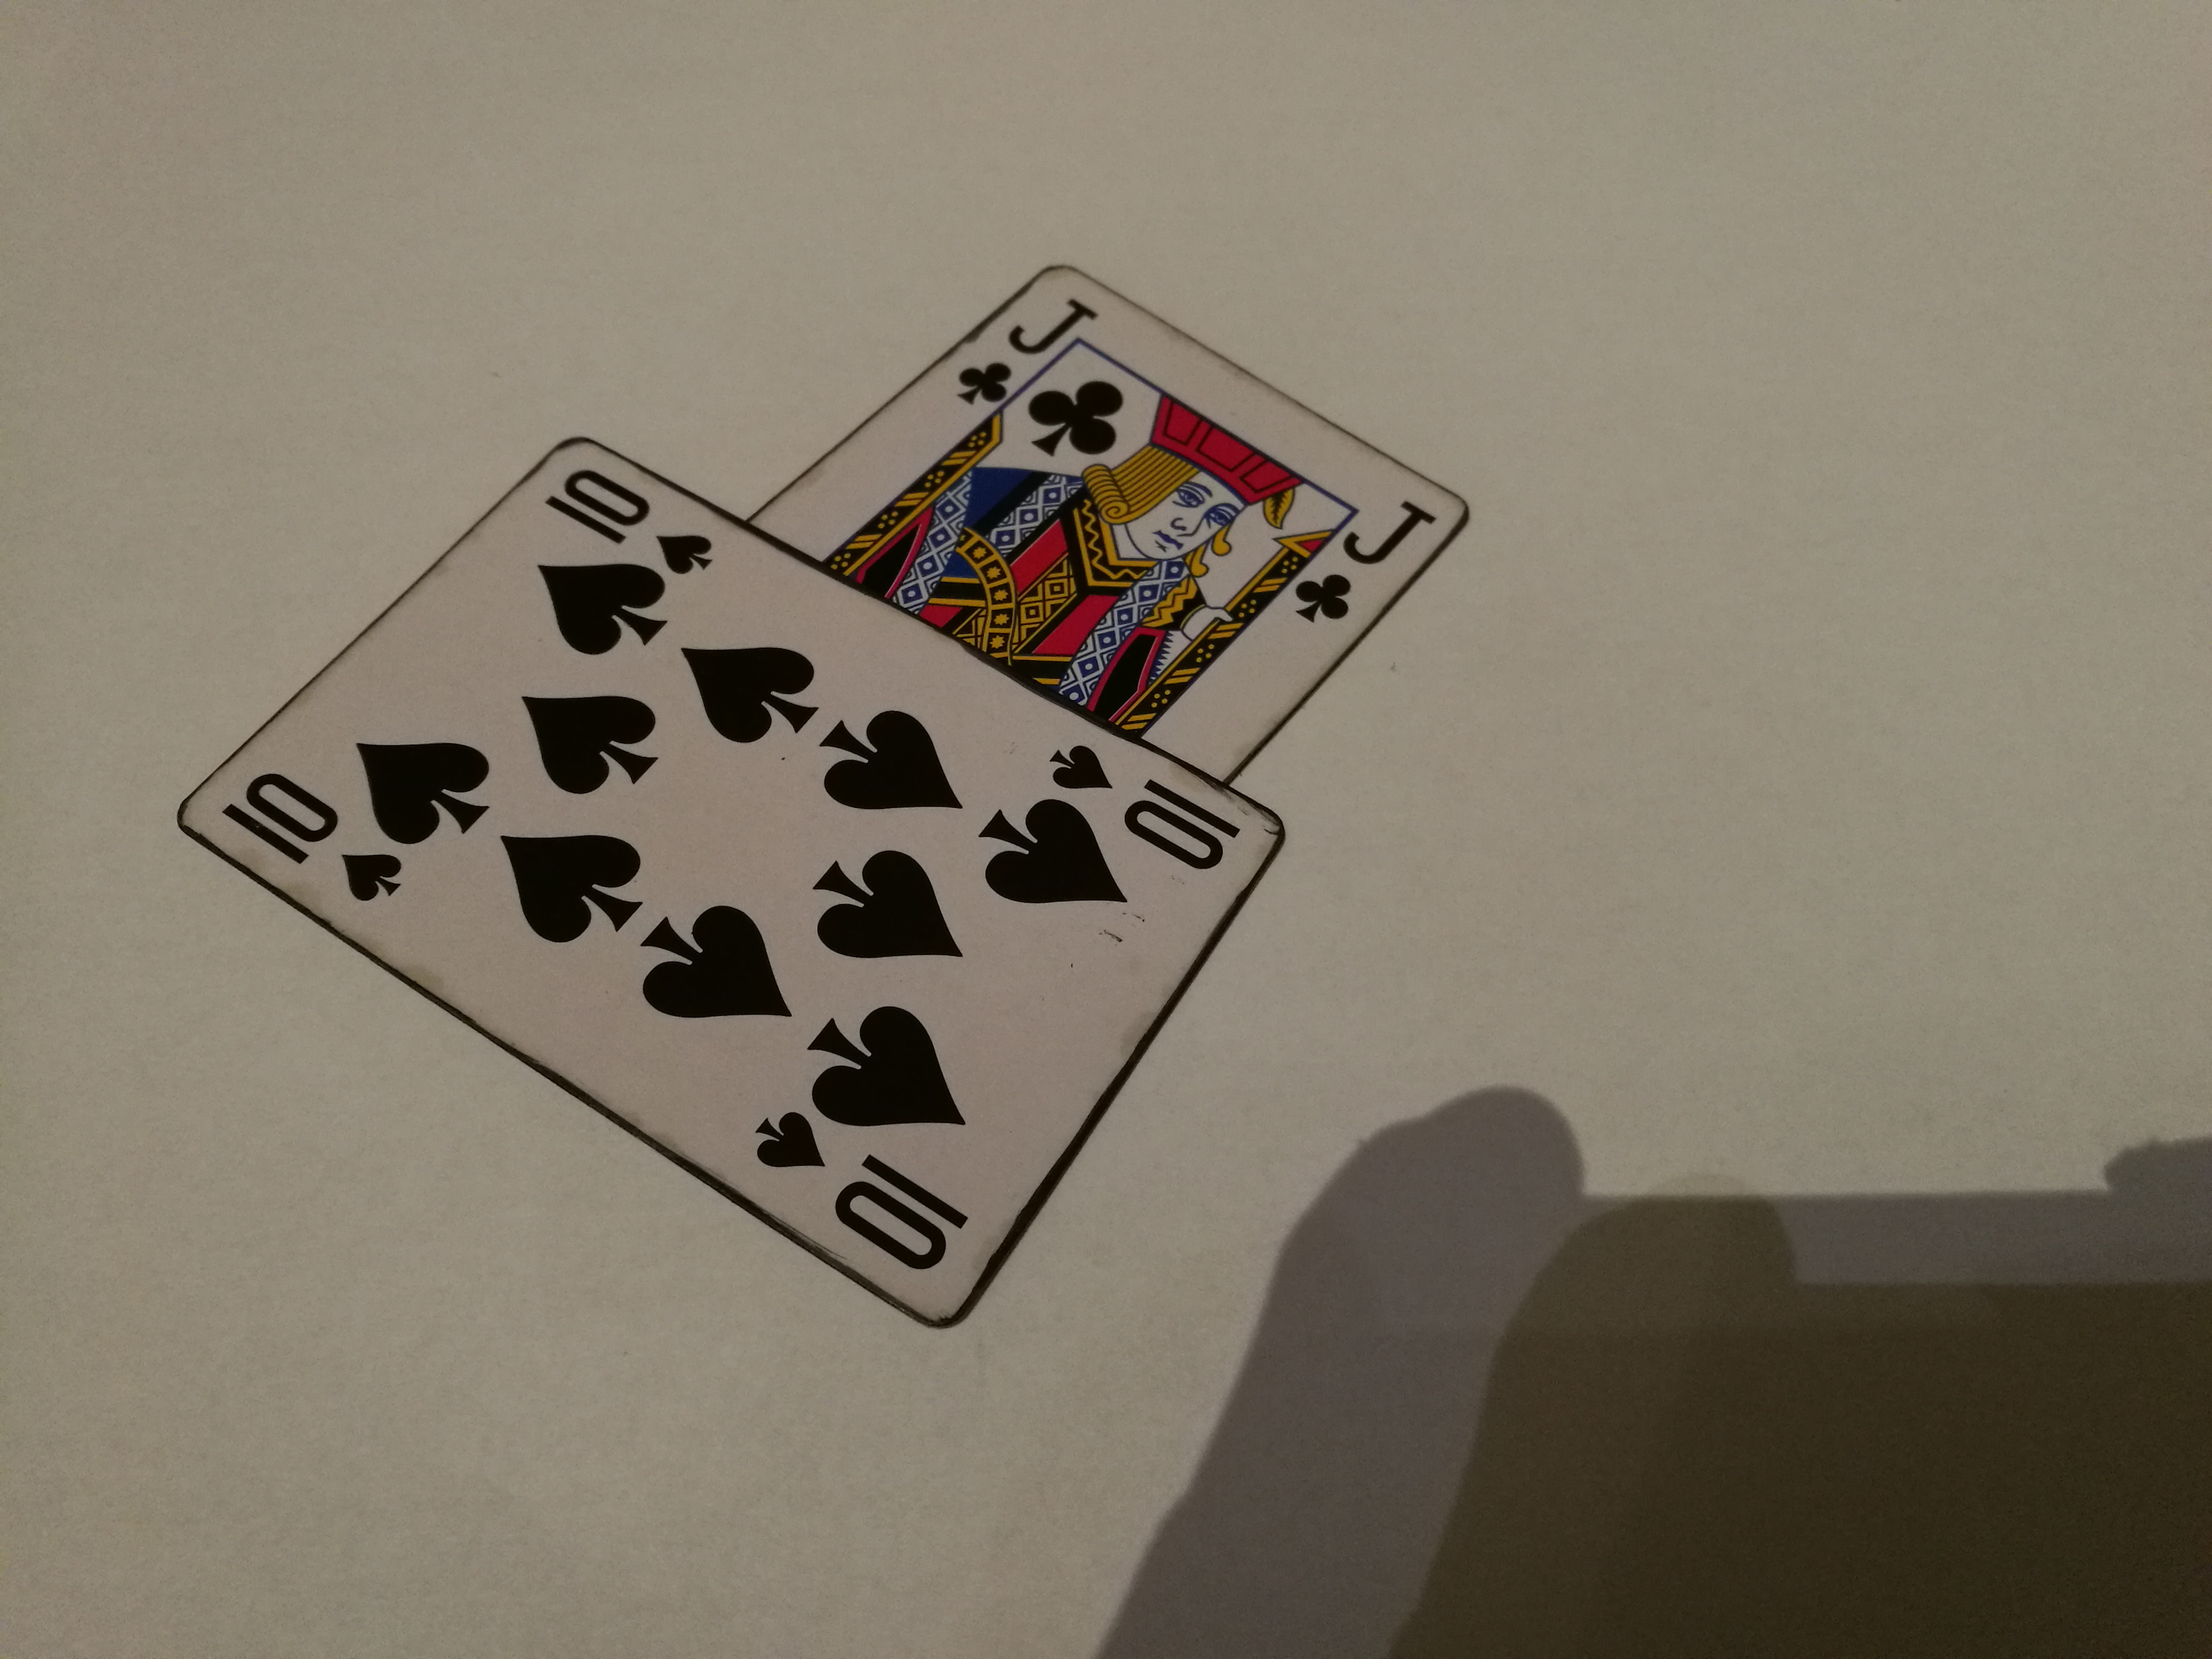
\includegraphics[width=0.4\textwidth]{datenbeispiel2.jpg}
 \caption{Kreuz-Bube sticht Pik-10, 12 Punkte gewonnen}
 \label{fig:img}
\end{figure}
\newpage
\section{Zeitplan}
\begin{table}[h!]
	\centering
		\begin{tabular}{|c|c|c|}
		\hline
		Meilenstein & abgeschlossen am & Arbeitsaufwand in h\\
		\hline
		Vorarbeit Projekt & 20.10.2017 & 20\\
		Prototyp erstellen& 10.11.2017 & 40\\
		Geometrische Transformation& 22.12.2017 & 105 \\
		Kantendetektion& 18.12.2017 & 67 \\
		Pattern-Matching & 18.12.2017 & 43\\
		GT-Test & 31.12.2017 & 10 \\
		KD-Test & 27.12.2017 & 5 \\
		PM-Test & 27.12.2017 & 5 \\
		Unit-Test & 05.01.2017 & 5 \\
		\hline
		\end{tabular}
\end{table}
\nocite{*}
\bibliographystyle{plain}
\bibliography{C:/Users/Thorsten/Documents/GitHub/EDBV/edbv_lit}{}
\end{document}
